\documentclass{beamer}
\usepackage{tikz}
\usepackage[orientation=landscape,size=a2,scale=1]{beamerposter}
\usepackage[absolute,overlay]{textpos}
\usetikzlibrary{arrows}
\begin{document}

\begin{textblock}{15}(0.5, 0.5)
    \begin{block}{}
        \centering
        \Large Suppression of Variation in Cell-Size: A Control Theoretic Approach \\
        \large Dilawar Singh, \texttt{dilawars@ncbs.res.in}
    \end{block}
    \begin{block}{Abstract}

        We propose a  possible mechanism based on control and information theory
        which can be used to control cell size. We explore few network
        topologies of a simple control network which can keep the size of the
        cell at a fixed value while giving a upper bound on the size of the
        Endosome.

\end{block}
\end{textblock}

\begin{textblock}{7}(0.5,3.5)

    \begin{block}{Network under study}
        \begin{figure}
            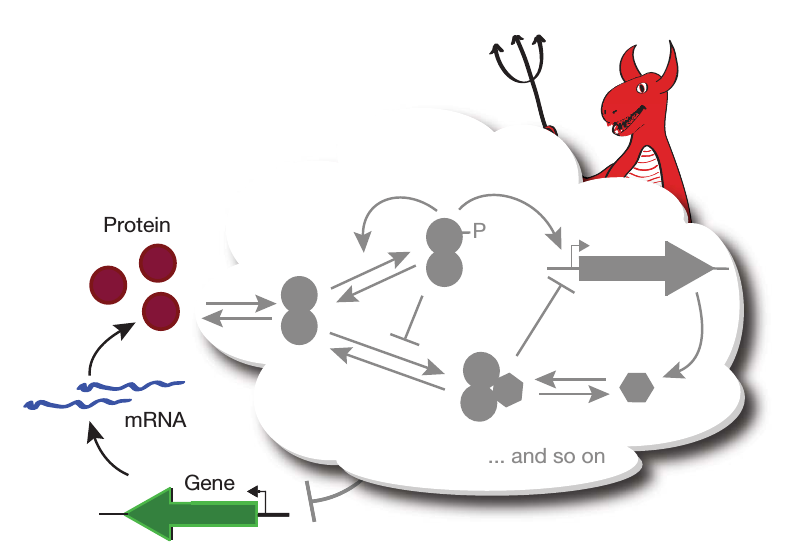
\includegraphics[]{./fig_mrna_protein.png}
%%        \begin{tikzpicture}[scale=1]
%%
%%            %% Here is the macro which draws the gene regulatory arrow.
%%            %% args: starting point, width, height, fillcolor
%%            \newcommand\arrow[4]
%%            {
%%                \draw[draw,fill=#4] #1 ++(0,{#3/4}) -- ++(0,{#3/2})
%%                -- ++({-#2*2/3},0) -- ++(0,{#3/4}) -- ++({-#2/3},{-#3/2})
%%                -- ++({#2/3},{-#3/2}) -- ++(0,{#3/4}) -- cycle
%%                ;
%%            };
%%
%%            \begin{scope}
%%                \arrow{(0,0)}{4}{2}{red};
%%            \end{scope}
%%
%%            
%%        \end{tikzpicture}
            \begin{tikzpicture}
                \node[] (x1) at (0,0) {$X_1$};
                \node[] (x2)  at (5,0) {$X_2$};
                \draw[->] (x1) -- (x2);
            \end{tikzpicture}
        \caption{Network under consideration. In our scheme $x_1$ is mRNA and
        $x_2$ is protein.}
        \label{fig:demon}
        \end{figure}
    
        \begin{equation}
            x_1 \rightarrow x_1 + 1 \\
        \end{equation}


    \end{block}

\end{textblock}

\end{document}
